\section{BCVTB Examples}\label{bcvtb-examples}

\subsection{Architecture of System}\label{architecture-of-system}

The figure below shows the architecture of the connection between EnergyPlus and the BCVTB. The black objects are explained in this application guide, whereas the grey items are not specific to EnergyPlus and are explained in the BCVTB documentation. The BCVTB connects to the external interface in EnergyPlus. In the external interface, the input/output signals that are exchanged between the BCVTB and EnergyPlus are mapped to EnergyPlus objects. The subject of this External Interface Application Guide is how to configure this mapping and how to use these objects. For a detailed explanation of the grey items, we refer to the BCVTB documentation.

\begin{figure}[hbtp] % fig 1
\centering
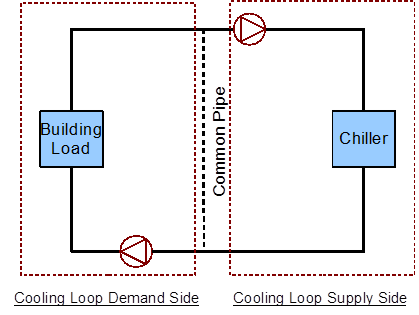
\includegraphics[width=0.9\textwidth, height=0.9\textheight, keepaspectratio=true]{media/image004.png}
\caption{Architecture of the BCVTB with the EnergyPlus client (black) and other clients (grey). \protect \label{fig:architecture-of-the-bcvtb-with-the-energyplus}}
\end{figure}

The external interface can map to three EnergyPlus input objects called ExternalInterface:Schedule, ExternalInterface:Actuator and ExternalInterface:Variable. The ExternalInterface:Schedule can be used to overwrite schedules, and the other two objects can be used in place of Energy Management System (EMS) actuators and EMS variables. The objects have similar functionality as the objects Schedule:Compact, EnergyManagementSystem:Actuator and EnergyManagementSystem:GlobalVariable, except that their numerical value is obtained from the external interface at the beginning of each zone time step, and will remain constant during this zone time step.

Compared to EnergyManagementSystem:Actuator, the object ExternalInterface:Actuator has an optional field called ``initial value.'' If a value is specified for this field, then this value will be used during the warm-up period and the system sizing. If unspecified, then the numerical value for this object will only be used during the time stepping. Since actuators always overwrite other objects (such as a schedule), all these objects have values that are defined during the warm-up and the system sizing even if no initial value is specified. For the objects~ ExternalInterface:Schedule and ExternalInterface:Variable, the field ``initial value'' is required, and its value will be used during the warm-up period and the system-sizing.

ExternalInterface:Variable is a global variable from the point of view of the EMS language. Thus, it can be used within any EnergyManagementSystem:Program in the same way as an EnergyManagementSystem:GlobalVariable or an EnergyManagementSystem:Sensor can be used.

Although variables of type ExternalInterface:Variable can be assigned to EnergyManagmentSystem:Actuator objects, for convenience, there is also an object called ExternalInterface:Actuator. This object behaves identically to EnergyManagmentSystem:Actuator, with the following exceptions:

\begin{itemize}
\item
  Its value is assigned by the external interface.
\item
  Its value is fixed during the zone time step because this is the synchronization time step for the external interface.
\end{itemize}

The external interface can also map to the EnergyPlus objects Output:Variable and EnergyManagementSystem:OutputVariable. These objects can be used to send data from EnergyPlus to the BCVTB at each zone time step.

We will now present examples that use all of these objects. The following table shows which EnergyPlus features are used in the examples, which are all distributed with the BCVTB installation that can be obtained from the LBNL web site. Note -- these examples are NOT distributed with EnergyPlus installation because you need the special software to make them work.

% table 1
\begin{longtable}[c]{@{}llll@{}}
\caption{Overview of the EnergyPlus objects used in Examples \label{table:overview-of-the-energyplus-objects-used-in}} \tabularnewline
\toprule 
~ & Example 1 & Example 2 & Example 3 \tabularnewline
\midrule
\endfirsthead

\caption[]{Overview of the EnergyPlus objects used in Examples} \tabularnewline
\toprule 
~ & Example 1 & Example 2 & Example 3 \tabularnewline
\midrule
\endhead

ExternalInterface:Schedule & x & ~ & ~ \tabularnewline
ExternalInterface:Actuator & ~ & X & ~ \tabularnewline
ExternalInterface:Variable & ~ & ~ & x \tabularnewline
Output:Variable & x & X & x \tabularnewline
EnergyManagementSystem:OutputVariable & ~ & ~ & x \tabularnewline
\bottomrule
\end{longtable}

To configure the data exchange, the following three steps are required from the user:

1)~~~Create an EnergyPlus idf file.

2)~~~Create an xml file that defines the mapping between EnergyPlus and BCVTB variables.

3)~~~Create a Ptolemy model.

These steps are described in the examples below. Prior to discussing the examples, we will explain the syntax of the xml configuration file that defines how data are mapped between the external interface and EnergyPlus.

\subsection{XML Syntax}\label{xml-syntax}

This section describes the syntax of the xml file that configures the data mapping between EnergyPlus and the external interface.

The data mapping between EnergyPlus and the external interface is defined in an xml file called variables.cfg. This file needs to be in the same directory as the EnergyPlus idf file.

The file has the following header:

\textless{}?xml version = ``1.0'' encoding = ``ISO-8859-1''?\textgreater{}

\textless{}!DOCTYPE BCVTB-variables SYSTEM ``variables.dtd''\textgreater{}

Following the header is an element of the form

\textless{}BCVTB-variables\textgreater{}

\textless{}/BCVTB-variables\textgreater{}

This element will contain child elements that define the variable mapping. In between the element tags, a user needs to specify how the exchanged data is mapped to EnergyPlus objects. Hence, the order of these elements matter, and it need to be the same as the order of the elements in the input and output signal vector of the BCVTB actor that calls EnergyPlus. The exchanged variables are declared in elements that are called ``variable'' and have an attribute ``source.'' As described above, the external interface can send data to ExternalInterface:Schedule, ExternalInterface:Actuator, ExternalInterface:Variable. For these objects, the ``source'' attribute needs to be set to ``Ptolemy,'' because they are computed in Ptolemy. The xml elements for these objects look as follows:

For ExternalInterface:Schedule, use

\textless{}variable source = ``Ptolemy''\textgreater{}

~~~ \textless{}EnergyPlus schedule = ``NAME''/\textgreater{}

~ \textless{}/variable\textgreater{}

where NAME needs to be the EnergyPlus schedule name. For ExternalInterface:Actuator, use

\textless{}variable source = ``Ptolemy''\textgreater{}

~~~ \textless{}EnergyPlus actuator = ``NAME'' /\textgreater{}

~ \textless{}/variable\textgreater{}

where NAME needs to be the EnergyPlus actuator name. For ExternalInterface:Variable, use

~ \textless{}variable source = ``Ptolemy''\textgreater{}

~~~ \textless{}EnergyPlus variable = ``NAME''/\textgreater{}

~ \textless{}/variable\textgreater{}

where NAME needs to be the EnergyPlus Energy Runtime Language (Erl) variable name.

The external interface can also read data from any Output:Variable and EnergyManagementSystem:OutputVariable. For these objects, set the ``source'' attribute to ``EnergyPlus,'' because they are computed by EnergyPlus. The read an Output:Variable, use

~ \textless{}variable source = ``EnergyPlus''\textgreater{}

~~~ \textless{}EnergyPlus name = ``NAME'' type = ``TYPE''/\textgreater{}

~ \textless{}/variable\textgreater{}

where NAME needs to be the EnergyPlus ``Variable Name'' (such as ZONE/SYS AIR TEMP) and TYPE needs to be the EnergyPlus ``Key Value'' (such as ZONE ONE). To read an EnergyManagementSystem:OutputVariable, use

\textless{}variable source = ``EnergyPlus''\textgreater{}

~~~ \textless{}EnergyPlus name = ``EMS'' type = ``TYPE''/\textgreater{}

\textless{}/variable\textgreater{}

i.e., the attribute ``name'' must be EMS, and the attribute ``type'' must be set to the EMS variable name.

Complete examples of these xml files are presented below.

\subsection{Example 1: Interface using ExternalInterface:Schedule}\label{example-1-interface-using-externalinterfaceschedule}

In this example, a controller that is implemented in the BCVTB computes the room temperature set points for cooling and heating. The example can be found in the BCVTB distribution in the folder examples/ePlusX-schedule, where X stands for the EnergyPlus version number.

Suppose we need to send from the BCVTB to EnergyPlus a schedule value, and from EnergyPlus to the BCVTB an output variable at each zone time step. This can be accomplished by using an object of type ExternalInterface:Schedule and an object of type Output:Variable.

To interface EnergyPlus using the EMS feature, the following three items are needed:

\begin{itemize}
\item
  An object that instructs EnergyPlus to activate the external interface.
\item
  EnergyPlus objects that write data from the external interface to the EMS.
\item
  A configuration file to configure the data exchange.
\end{itemize}

\subsubsection{Creating the EnergyPlus idf file}\label{creating-the-energyplus-idf-file}

The EnergyPlus idf file contains the following objects to activate and use the external interface:

\begin{itemize}
\item
  An object that instructs EnergyPlus to activate the external interface.
\item
  An object of type ExternalInterface:Schedule. The external interface will write its values to these objects at each zone time-step.
\item
  Objects of type Output:Variable. Any EnergyPlus output variable can be read by the external interface.
\end{itemize}

The code below shows how to declare these objects.

To activate the external interface, we use:

\begin{lstlisting}

ExternalInterface,           !- Object to activate the external interface
   PtolemyServer;              !- Name of external interface
\end{lstlisting}

To enter schedules to which the external interface writes, we use:

\begin{lstlisting}

! Cooling schedule. This schedule is set directly by the external interface.
  ! During warm-up and system-sizing, it is fixed at 24 degC.
    ExternalInterface:Schedule,
      TSetCoo,                 !- Name
      Temperature,             !- ScheduleType
      24;                      !- Initial value, used during warm-up


  ! Heating schedule. This schedule is set directly by the external interface.
  ! During warm-up and system-sizing, it is fixed at 20 degC.
    ExternalInterface:Schedule,
      TSetHea,                 !- Name
      Temperature,             !- ScheduleType
      20;                      !- Initial value, used during warm-up
\end{lstlisting}

These schedules can be used as other EnergyPlus schedules. In this example, they are used to change a thermostat setpoint:

\begin{lstlisting}

ThermostatSetpoint:DualSetpoint,
      DualSetPoint,            !- Name
      BCVTB-SP-TH,             !- Heating Setpoint Temperature Schedule Name
      BCVTB-SP-TC;             !- Cooling Setpoint Temperature Schedule Name
\end{lstlisting}

We also want to read from EnergyPlus output variables, which we declare as

\begin{lstlisting}

Output:Variable,
      TSetHea,        !- Key Value
      Schedule Value, !- Variable Name
      TimeStep;       !- Reporting Frequency


  Output:Variable,
      TSetCoo,        !- Key Value
      Schedule Value, !- Variable Name
      TimeStep;       !- Reporting Frequency
\end{lstlisting}

To specify that data should be exchanged every 15 minutes of simulation time, enter in the idf file the section

\begin{lstlisting}

  Timestep,
      4;          !- Number of Timesteps per Hour
\end{lstlisting}

\subsubsection{Creating the configuration file}\label{creating-the-configuration-file}

Note that we have not yet specified the order of the elements in the signal vector that is exchanged between EnergyPlus and the BCVTB. This information is specified in the file variables.cfg. The file variables.cfg needs to be in the same directory as the EnergyPlus idf file. For the objects used in the section above, the file looks like

\begin{lstlisting}

<?xml version = "1.0" encoding = "ISO-8859-1"?>
  <!DOCTYPE BCVTB-variables SYSTEM "variables.dtd">
  <BCVTB-variables>
    <!-- The next two elements send the set points to E+ -->
    <variable source = "Ptolemy">
      <EnergyPlus schedule = "TSetHea"/>
    </variable>
    <variable source = "Ptolemy">
      <EnergyPlus schedule = "TSetCoo"/>
    </variable>
    <!-- The next two elements receive the outdoor and zone air temperature from E+ -->
    <variable source = "EnergyPlus">
     <EnergyPlus name = "ENVIRONMENT" type = "SITE OUTDOOR AIR DRYBULB TEMPERATURE"/>
    </variable>
    <variable source = "EnergyPlus">
      <EnergyPlus name = "ZSF1" type = "ZONE AIR TEMPERATURE"/>
    </variable>
    <!-- The next two elements receive the schedule value as an output from E+ -->
    <variable source = "EnergyPlus">
      <EnergyPlus name = "TSetHea" type = "Schedule Value"/>
    </variable>
    <variable source = "EnergyPlus">
      <EnergyPlus name = "TSetCoo" type = "Schedule Value"/>
    </variable>
  </BCVTB-variables>
\end{lstlisting}

This file specifies that the actor in the BCVTB that calls EnergyPlus has an input vector with two elements that are computed by Ptolemy (Ptolemy is the name of the software on which the BCVTB is based) and sent to EnergyPlus, and that it has an output vector with four elements that are computed by EnergyPlus and sent to Ptolemy. The order of the elements in each vector is determined by the order in the above XML file. Hence, the input vector that contains the signals sent to EnergyPlus has elements

TSetHea

~ TSetCoo

and the output vector that contains values computed by EnergyPlus has elements

Environment (Site Outdoor Air Drybulb Temperature)

~ ZSF1 (ZONE AIR TEMPERATURE)

~ TSetHea (Schedule Value)

~ TSetCoo (Schedule Value)

\paragraph{\textbf{Creating the Ptolemy model}}\label{creating-the-ptolemy-model}

To start EnergyPlus from the BCVTB, you will need to create a Ptolemy model.

The model bcvtb/example/ePlus40-schedule/system-windows.xml that is part of the BCVTB installation and that is shown below may be used as a starting point. (For Mac and Linux, use the file system.xml.) In this example, the time step is 15 minutes and the simulation period is four days.

\begin{figure}[hbtp] % fig 2
\centering
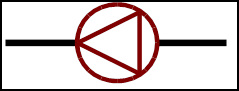
\includegraphics[width=0.9\textwidth, height=0.9\textheight, keepaspectratio=true]{media/image005.png}
\caption{System model in the BCVTB. \protect \label{fig:system-model-in-the-bcvtb.}}
\end{figure}

In this model, the Simulator actor that calls EnergyPlus is configured for Windows as follows:

\begin{figure}[hbtp] % fig 3
\centering
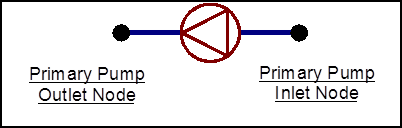
\includegraphics[width=0.9\textwidth, height=0.9\textheight, keepaspectratio=true]{media/image006.png}
\caption{Configuration of the Simulator actor that calls EnergyPlus on Windows. \protect \label{fig:configuration-of-the-simulator-actor-that}}
\end{figure}

Hence, it calls the file ``RunEPlus.bat,'' with arguments ``EMSWindowShadeControl USA\_IL\_Chicago-OHare.Intl.AP.725300\_TMY3.'' The working directory is the current directory and the console output is written to the file simulation.log. If EnergyPlus does not communicate with the BCVTB within 10 seconds, the BCVTB will terminate the connection. (See \url{http://simulationresearch.lbl.gov/bcvtb} for more detailed documentation about how to configure a BCVTB model that communicates with other programs.)

For Mac OS X and Linux, the configuration is similar:

\begin{figure}[hbtp] % fig 4
\centering
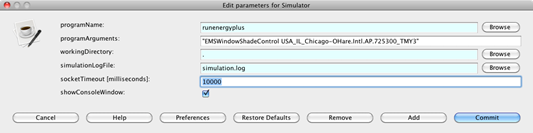
\includegraphics[width=0.9\textwidth, height=0.9\textheight, keepaspectratio=true]{media/image007.png}
\caption{Configuration of the Simulator actor that calls EnergyPlus on Mac OS X and on Linux. \protect \label{fig:configuration-of-the-simulator-actor-that-001}}
\end{figure}

This completes the configuration.

\subsection{Example 2: Interface using ExternalInterface:Actuator}\label{example-2-interface-using-externalinterfaceactuator}

In this example, a shading controller with a finite state machine is implemented in the BCVTB. Inputs to the controller are the outside temperature and the solar radiation that is incident on the window. The output of the controller is the shading actuation signal.

This example describes how to set up EnergyPlus to exchange data between the BCVTB and EnergyPlus, using an Energy Management System (EMS) actuator. The example can be found in the BCVTB distribution in the folder examples/ePlusX-actuator, where X stands for the EnergyPlus version number.

The object of type ExternalInterface:Actuator behaves identically to EnergyManagmentSystem:Actuator, with the following exceptions:

\begin{itemize}
\item
  Its value is assigned by the external interface.
\item
  Its value is fixed during the zone time step because this is the synchronization time step for the external interface.
\end{itemize}

To interface EnergyPlus using the EMS feature, the following three items are needed:

1)~~~An object that instructs EnergyPlus to activate the external interface.

2)~~~EnergyPlus objects that write data from the external interface to the EMS.

3)~~~A configuration file to configure the data exchange.

\subsubsection{Creating the EnergyPlus idf file}\label{creating-the-energyplus-idf-file-1}

The code below shows how to set up an EnergyPlus file that uses EnergyManagmentSystem:Actuator. To activate the external interface, we use:

\begin{lstlisting}

ExternalInterface,           !- Object to activate the external interface
   PtolemyServer;              !- Name of external interface
\end{lstlisting}

To declare an actuator that changes the control status of the window with name ``Zn001:Wall001:Win001'', we use:

\begin{lstlisting}

ExternalInterface:Actuator,
      Zn001_Wall001_Win001_Shading_Deploy_Status,  !- Name
      Zn001:Wall001:Win001,    !- Actuated Component Unique Name
      Window Shading Control,  !- Actuated Component Type
      Control Status,          !- Actuated Component Control Type
       ;                       ! initial value
\end{lstlisting}

Thus, the entry is identical with EnergyManagmentSystem:Actuator, except for the additional optional field that specifies the initial value. If unspecified, then the actuator will only be used during the time stepping, but not during the warm-up and the system sizing. Since actuators always overwrite other objects (such as a schedule), all these objects have values that are defined during the warm-up and the system sizing even if no initial value is specified.

We also want to read from EnergyPlus the outdoor temperature, the zone air temperature, the solar radiation that is incident on the window, and the fraction of time that the shading is on. Thus, we declare the output variables

\begin{lstlisting}

Output:Variable,
     Environment,                            !- Key Value
     Site Outdoor Air Drybulb Temperature,   !- Variable Name
     timestep;                               !- Reporting Frequency


  Output:Variable,
     *,                                      !- Key Value
     Zone Mean Air Temperature,              !- Variable Name
     timestep;                               !- Reporting Frequency


  Output:Variable,
     Zn001:Wall001:Win001,                   !- Key Value
     Surface Outside Face Incident Solar Radiation Rate per Area, !- Var Name
     timestep;                               !- Reporting Frequency


  Output:Variable,
     *,                                      !- Key Value
     Surface Shading Device Is On Time Fraction,  !- Variable Name
     timestep;                               !- Reporting Frequency
\end{lstlisting}

To specify that data should be exchanged every 10 minutes of simulation time, we enter in the idf file the section

\begin{lstlisting}

  Timestep,
      6;          !- Number of Timesteps per Hour
\end{lstlisting}

\paragraph{\textbf{Creating the configuration file}}\label{creating-the-configuration-file-1}

Note that we have not yet specified the order of the elements in the signal vector that is exchanged between EnergyPlus and the BCVTB. This information is specified in the file variables.cfg. The file variables.cfg needs to be in the same directory as the EnergyPlus idf file. For the objects used in the section above, the file looks like

\begin{lstlisting}

<?xml version = "1.0" encoding = "ISO-8859-1"?>
  <!DOCTYPE BCVTB-variables SYSTEM "variables.dtd">
  <BCVTB-variables>
    <variable source = "EnergyPlus">
     <EnergyPlus name = "ENVIRONMENT" type = "SITE OUTDOOR AIR DRYBULB TEMPERATURE"/>
    </variable>
    <variable source = "EnergyPlus">
      <EnergyPlus name = "WEST ZONE" type = "Zone Mean Air Temperature"/>
    </variable>
    <variable source = "EnergyPlus">
      <EnergyPlus name = "Zn001:Wall001:Win001" type = "Surface Outside Face Incident Solar Radiation Rate per Area"/>
    </variable>
    <variable source = "EnergyPlus">
      <EnergyPlus name = "Zn001:Wall001:Win001" type = "Surface Shading Device Is On Time Fraction"/>
    </variable>
    <variable source = "Ptolemy">
      <EnergyPlus actuator = "Zn001_Wall001_Win001_Shading_Deploy_Status" />
    </variable>
  </BCVTB-variables>
\end{lstlisting}

This file specifies that the actor in the BCVTB that calls EnergyPlus has an input vector with one element that will be written to the actuator, and that it has an output vector with four elements that are computed by EnergyPlus and sent to Ptolemy. The order of the elements in each vector is determined by the order in the above XML file. Hence, the output vector that contains the signals computed by EnergyPlus has elements

\begin{lstlisting}
  ENVIRONMENT (SITE OUTDOOR AIR DRYBULB TEMPERATURE)
  WEST ZONE (Zone Mean Air Temperature)
  Zn001:Wall001:Win001 (Surface Outside Face Incident Solar Radiation Rate per Area)
  Zn001:Wall001:Win001 (Surface Shading Device Is On Time Fraction)
\end{lstlisting}

The configuration of the Ptolemy model is identical to the configuration in Example 1.

\subsection{Example 3: Interface using ExternalInterface:Variable}\label{example-3-interface-using-externalinterfacevariable}

This example implements the same controller as the Example 2. However, the interface with EnergyPlus is done using an external interface variable instead of an external interface actuator. In addition, the example uses an EnergyManagementSystem:OutputVariable to set up data that will be read by the external interface.

Similarly to EnergyManagementSystem:GlobalVariable, an ExternalInterface:Variable can be used in any EnergyManagementSystem:Program. The subject of this example is to illustrate how an ExternalInterface:Variable can be set up for use in an EnergyManagementSystem:Program. The example can be found in the BCVTB distribution in the folder examples/ePlusX-variable, where X stands for the EnergyPlus version number.

To interface EnergyPlus using an external interface variable, the following items are needed:

\begin{itemize}
\item
  An object that instructs EnergyPlus to activate the external interface.
\item
  EnergyPlus objects that write data from the external interface to the EMS.
\item
  A configuration file to configure the data exchange.
\end{itemize}

\subsubsection{Creating the EnergyPlus idf file}\label{creating-the-energyplus-idf-file-2}

To write data from the external interface to an EnergyPlus EMS variable, an EnergyPlus object of the following entry may be used in the idf file:

\begin{lstlisting}

ExternalInterface,           !- Object to activate the external interface
     PtolemyServer;            !- Name of external interface


    ExternalInterface:Variable,
      yShade,                  !- Name of Erl variable
      1;                       !- Initial value
\end{lstlisting}

During the warm-up period and the system-sizing, the variable will be set to its initial value. Afterwards, the value will be assigned from the external interface at each beginning of a zone time step and kept constant during the zone time step. From the point of view of the EMS language, ExternalInterface:Variable can be used like any global variable. Thus, it can be used within any EnergyManagementSystem:Program in the same way as an EnergyManagementSystem:GlobalVariable or an EnergyManagementSystem:Sensor.

This idf section above activates the external interface and declares a variable with name yShade that can be used in an Erl program to actuate the shading control of the window ``Zn001:Wall001:Win001'' as follows:

\begin{lstlisting}

! EMS program. The first assignments sets the shading status and converts it into the
  !              EnergyPlus signal (i.e., replace 1 by 6).
  !              The second assignment sets yShade to
  !              an EnergyManagementSystem:OutputVariable
  !              which will be read by the external interface.
    EnergyManagementSystem:Program,
      Set_Shade_Control_State,          !- Name
      Set Shade_Signal = 6*yShade,      !- Program Line 1
      Set Shade_Signal_01 = yShade+0.1; !- Program Line 2


  ! Declare an actuator to which the EnergyManagementSystem:Program will write
    EnergyManagementSystem:Actuator,
      Shade_Signal,  !- Name
      Zn001:Wall001:Win001,             !- Actuated Component Unique Name
      Window Shading Control,           !- Actuated Component Type
      Control Status;                   !- Actuated Component Control Type


  ! Declare a global variable to which the EnergyManagementSystem:Program will write
    EnergyManagementSystem:GlobalVariable,
      Shade_Signal_01;                  !- Name of Erl variable
\end{lstlisting}

We want to read from EnergyPlus the outdoor temperature, the zone air temperature and the solar radiation that is incident on the window. Thus, we declare

\begin{lstlisting}

Output:Variable,
     Environment,                 !- Key Value
     Site Outdoor Air Drybulb Temperature,            !- Variable Name
     timestep;                    !- Reporting Frequency


    Output:Variable,
    *,                          !- Key Value
    Zone Mean Air Temperature,  !- Variable Name
    timestep;                   !- Reporting Frequency


    Output:Variable,
    Zn001:Wall001:Win001,       !- Key Value
    Surface Outside Face Incident Solar Radiation Rate per Area, !- Var Name
    timestep;                   !- Reporting Frequency
\end{lstlisting}

In addition, we want to output the variable ``Erl Shading Control Status'' that has been set up as

\begin{lstlisting}

! Declare an output variable. This variable is equal to the shahing signal + 0.1
  ! It will be reah by the external interface to hemonstrate how to receive variables.
    EnergyManagementSystem:OutputVariable,
      Erl Shahing Control Status,  !- Name
      Shahe_Signal_01,             !- EMS Variable Name
      Averageh,                    !- Type of Data in Variable
      ZoneTimeStep;                !- Uphate Frequency
\end{lstlisting}

To specify that data should be exchanged every 10 minutes of simulation time, enter in the idf file the section

\begin{lstlisting}

  Timestep,
      6;          !- Number of Timesteps per Hour
\end{lstlisting}

\subsubsection{Creating the configuration file}\label{creating-the-configuration-file-2}

Note that we have not yet specified the order of the elements in the signal vector that is exchanged between EnergyPlus and the BCVTB. This information is specified in the file variables.cfg. The file variables.cfg needs to be in the same directory as the EnergyPlus idf file. For the objects used in the section above, the file looks like

\begin{lstlisting}

<?xml version = "1.0" encoding = "ISO-8859-1"?>
  <!DOCTYPE BCVTB-variables SYSTEM "variables.dtd">
  <BCVTB-variables>
    <variable source = "Ptolemy">
      <EnergyPlus variable = "yShade"/>
    </variable>
    <variable source = "EnergyPlus">
      <EnergyPlus name = "ENVIRONMENT" type = "SITE OUTDOOR AIR DRYBULB TEMPERATURE"/>
    </variable>
    <variable source = "EnergyPlus">
      <EnergyPlus name = "WEST ZONE" type = "Zone Mean Air Temperature"/>
    </variable>
    <variable source = "EnergyPlus">
      <EnergyPlus name = "Zn001:Wall001:Win001" type = "Surface Outside Face Incident Solar Radiation Rate per Area"/>
    </variable>
    <variable source = "EnergyPlus">
      <EnergyPlus name = "EMS" type = "Erl Shading Control Status"/>
    </variable>
  </BCVTB-variables>
\end{lstlisting}

This file specifies that the actor in the BCVTB that calls EnergyPlus has an input vector with one element that will be written to the actuator, and that it has an output vector with four elements that are computed by EnergyPlus and sent to Ptolemy. The order of the elements in each vector is determined by the order in the above XML file. Note that the fourth element has the name ``EMS'' because it is an EnergyManagementSystem:OutputVariable. Hence, the output vector that contains the signals computed by EnergyPlus has elements

\begin{lstlisting}
  ENVIRONMENT (SITE OUTDOOR AIR DRYBULB TEMPERATURE)
  WEST ZONE (Zone Mean Air Temperature)
  Zn001:Wall001:Win001 (Surface Outside Face Incident Solar Radiation Rate per Area)
  EMS (Erl Shading Control Status)
\end{lstlisting}

The configuration of the Ptolemy model is identical to the configuration in the previous examples.
